
\section{Simulation flow follow-up \ddcnew}
\label{chap5_newFlow}

%\begin{figure}[ht]
%    \centering
%    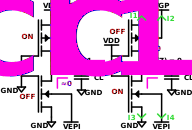
\includegraphics[width=0.5\textwidth]{5_faultModel/figures/ivx3NewNoSignals.pdf}
%    \caption{PLACEHOLDER.}
%    \label{fig_ivxNoSig}
%\end{figure}

\begin{figure}[ht]
    \centering
    \begin{subfigure}{0.47\textwidth}
        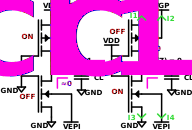
\includegraphics[width=1.0\textwidth, center]{5_faultModel/figures/ivx3NewNoSignals.pdf}
        \caption{PLACEHOLDER.}
        \label{fig_ivxNoSig}
    \end{subfigure}
    \hfill
    \begin{subfigure}{0.47\textwidth}
        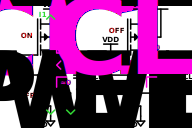
\includegraphics[width=1.0\textwidth, center]{5_faultModel/figures/ivx3New.pdf}
        \caption{PLACEHOLDER.}
        \label{fig_ivxSig}
    \end{subfigure}
    \caption{PLACEHOLDER.}
    \label{fig_ivxSim}
\end{figure}

The main shortcoming of the simulation flow presented in chapter \ref{chap:3icModeling} lies in the fact that the models do not consider the logic functions of the considered ICs.
To that end, I introduce in this section a way to circumvent this limitation.
As the \scs models are made for a specific technology, in that case for a 90 nm bulk silicon manufacturing process, the models parameters are calculated according to this technology node.
In addition to this, a single \scs model represents a hundred of logic gates.
Therefore, the disturbances observed in a \scs elementary block are the ones these logic gates would be subject to during \bbi.
With this in mind, I chose a very simple method of using the data from \scs simulations.

It consists in modeling actual transistors and logic gates with the considered technology and simulating them using the extracted disturbances from the \scs simulation results.
For the purpose of this work, I chose to simulate inverters in two specific scenarios:
\begin{itemize}
    \setlength\itemsep{-0.1em}
    \item A normally low inverter, fed with a logical high signal at its input;
    \item A normally high inverter, fed with a logical low signal at its input.
\end{itemize}


\begin{figure}[ht]
    \centering
    \begin{subfigure}{0.48\textwidth}
        \includegraphics[width=1.0\textwidth, center]{5_faultModel/figures/logic_gates_solo_M0_DW.pdf}
        \caption{PLACEHOLDER.}
        \label{fig_ivxDual}
    \end{subfigure}
    \hfill
    \begin{subfigure}{0.48\textwidth}
        \includegraphics[width=1.0\textwidth, center]{5_faultModel/figures/logic_gates_solo_M0_TW.pdf}
        \caption{PLACEHOLDER.}
        \label{fig_ivxTriple}
    \end{subfigure}
    \caption{PLACEHOLDER.}
    \label{fig_ivxSimRes}
\end{figure}
